\section{Rarefied gas flows}

\subsection{The Knudsen number}
For gases we define their \textit{Mean Free Path} as the average distance that 
the molecules of this gas are traveling without taking part in collisions.
The MFP of a hard-sphere gas in thermodynamic equilibrium is given by the equation:
\begin{equation}
 \lambda = \frac{1}{\sqrt{2} \pi \cdot n_\mathrm{g} \cdot d^2}
 \label{eq:MFP}
\end{equation}
where $d$ is the mean molecular diameter and $n_\mathrm{g}$ the number density of the gas~\cite{Zhang2012}.
Referring to the mean molecular spacing as $\delta$, $n_\mathrm{g}=\delta^{-3}$.
For air at atmospheric conditions ($T=298\,\mathrm{K}$, $p=1\,\mathrm{atm}$),
$\lambda_{\mathrm{air}} = 6.111\cdot10^{-8}\,\mathrm{m}$
while for the (lighter and smaller) helium 
$\lambda_{\mathrm{He}} = 17.651\cdot10^{-8}\,\mathrm{m}$~\cite{Karniadakis_Microflows}.

Knowing the MFP of a gas we can compute the \textit{Knudsen number} for a given scale.
This is defined as the ratio of the MFP to the characteristic length $L_0$ of the geometry:
\begin{equation}
 \mathrm{Kn} := \frac{\lambda}{L_0}
 \label{eq:Kn_def}
\end{equation}
The length $L_0$ can also be a limit above which very large variations of a macroscopic
quantity $\Phi_0$ may be observed and we can also write:
\begin{equation}
 \mathrm{Kn} \approx \frac{\lambda}{\Phi_0} \cdot \Big|\frac{\mathrm{d}\Phi_0}{\mathrm{d}L_0}\Big|
 \label{eq:Kn_phi}
\end{equation}
In complex geometries, a local Knudsen number can be chosen to solve the problem
of deciding about the characteristic length.
Equation~\ref{eq:Kn_phi} gives a good intuition for the relevance of the Knudsen number with
the continuity assumption, as in ``continuous'' scenarios (small $\mathrm{Kn}$) we would expect small
variations of macroscopic quantities. We can also relate the
Knudsen number to the Mach and Reynolds numbers:
\begin{equation}
 \mathrm{Kn} = \frac{\lambda}{L_0} \cdot \sqrt{\frac{\pi \gamma}{2}} \cdot \frac{\mathrm{Ma}}{\mathrm{Re}}
 \label{eq:Kn_Ma}
\end{equation}
where $\gamma := c_p / c_V$ is the specific heat capacity ratio of the gas~\cite{Zhang2012}.



\subsection{Division of the gas flow regimes}
The Knudsen number can be used to divide different \textit{flow regimes} and a
rough, empirical classification can be found in figure~\ref{fig:flow_regimes},
though it has been shown that Knudsen number is not the only parameter that needs
to be taken into account~\cite{Barber2006}.
The region $\mathrm{Kn}<10^{-2}$ (or $\mathrm{Kn}<10^{-3}$, as more recently suggested)
is referred to as the \textit{continuum regime}, in which all the required
assumptions hold, so that the application of the Navier-Stokes equations with the usual
no-slip boundary conditions is valid.
The other part of the range, where $\mathrm{Kn}>10$, corresponds to the
\textit{free molecular regime}. In this area, the molecules almost do not collide
with each other.
In between, the gas flow may belong to the \textit{slip-flow regime}
($10^{-2} < \mathrm{Kn} < 10^{-1} $) or to the \textit{transition regime}
($10^{-1} < \mathrm{Kn} < 10 $). 

Which regimes are mainly of practical interest? The term \textit{Rarefied Gas Flows} 
usually refers to the slip-flow and the
transition regime. As an example, $\mathrm{Kn}=1$ for air 
is achieved around length scale $L_0 = 65\,\mathrm{nm}$.
In some applications, different scales and flow regimes may be paired (\textit{mixed flow regimes}),
leading to the need of studying transport phenomena in a wide Knudsen range~\cite{Karniadakis_Microflows}.

\begin{figure}[h!]%
 	\begin{center}%
 		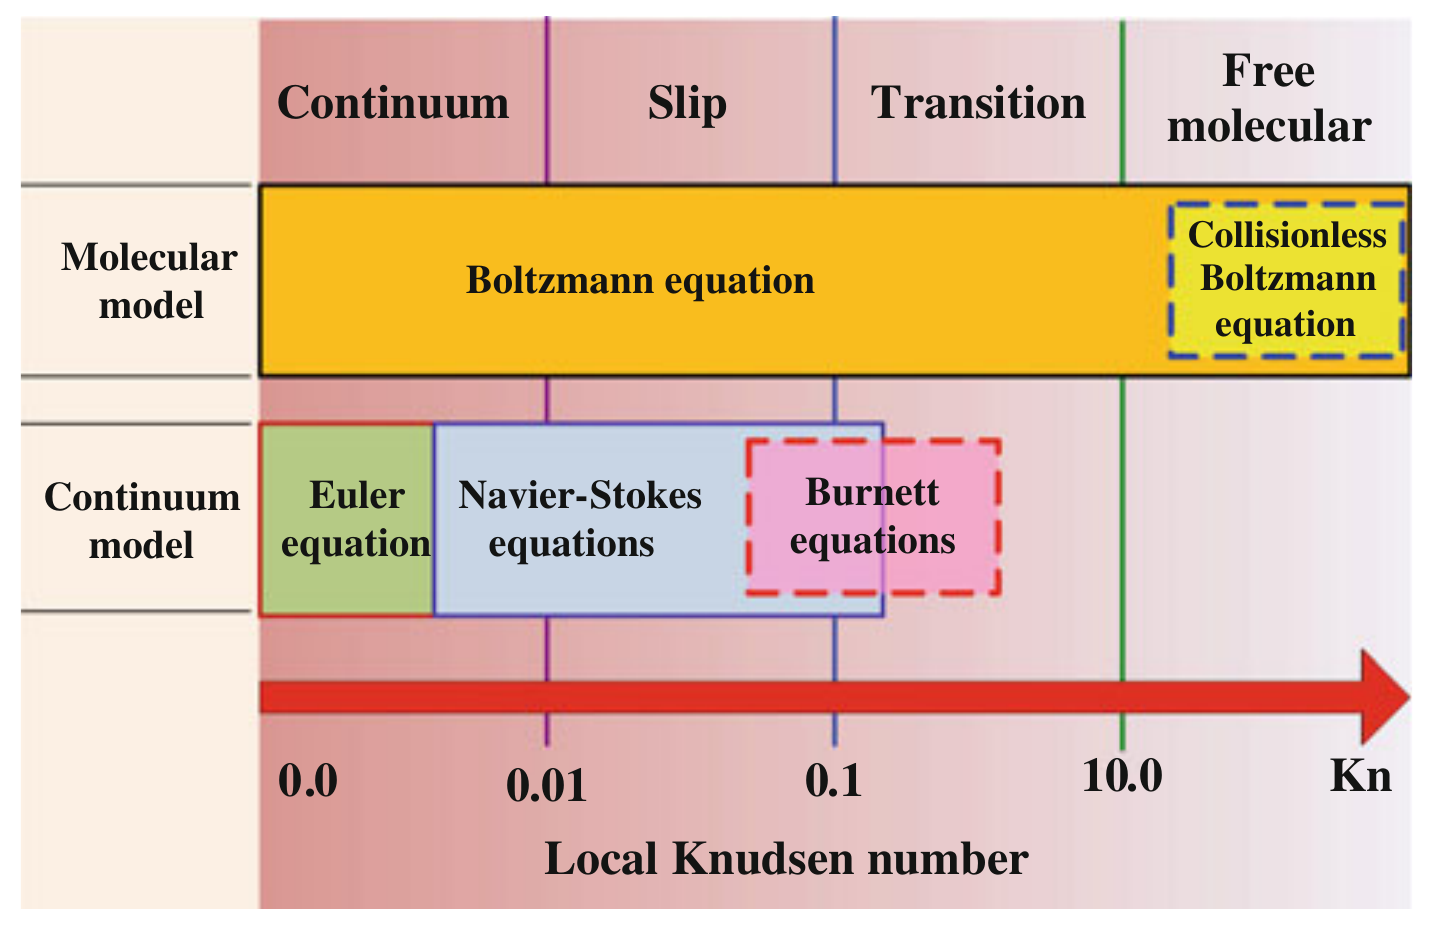
\includegraphics[scale=0.2]{flow_regimes}%
 		\caption{Division of the gas flow regimes in relation to the Knudsen %
 		number, along with the limits of different CFD %
 		approaches.~\cite{Zhang2012}}%
 		\label{fig:flow_regimes}%
 	\end{center}%
\end{figure}

\subsection{Where the continuous methods break}
The Navier-Stokes equations describe the conservation of mass and momentum in
the system. Adding the conservation of energy, we have the Navier-Stokes-Fourier
equations that require the following assumptions~\cite{Barber2006}:
\begin{description}
 \item[Newtonian Framework] The characteristic velocity has to be much smaller than the speed of light.
 This assumption is usually satisfied in the problems of our interest.
 \item[Continuum approximation] The fluid is infinitely divisible. This means that
 properties like the pressure, the velocity and the shear stress can be defined locally as averages between
 neighboring cells of a mesh. This assumption depends on the Knudsen number and it mainly does \textit{not} hold in our problems.
 \item[Thermodynamic equilibrium] The particles of the system have enough time to reach
 an equilibrium, by colliding with each other and relaxing the values of their properties.
 This depends on the frequency of the collisions and thus the Knudsen number.
\end{description}

It is suggested that the ratio $L_0/\delta$ should be greater than 100 in order
to achieve statistically stable estimate of macroscopic quantities
(limit of molecular chaos) and thus to assume continuity~\cite{Barber2006}.
Starting from the continuum regime, an increase in the Knudsen number breaks
the thermodynamic equilibrium assumption at around $\mathrm{Kn}=10^{-3}$,
as temperature jumps start to occur between the molecules and the walls,
forcing the gas to ``slip'' on the wall, i.e., the velocity near the wall cannot
be assumed as zero and the mass flux increases.
In the slip regime, the continuous methods can still be applied, combined with slip-velocity
and temperature-jump boundary conditions. In the transition regime,
a non-linear stress-strain relationship is observed for the fluid near the walls.
This area, that has width of a few MFP, is called \textit{``Knudsen layer''}. The 
continuum assumption breaks down and the NSF equations cannot be applied, while
the lattice Boltzmann method must be extended.
